\documentclass[t,linespread=1.2]{ctexbeamer}

\usepackage[size=a4,orientation=portrait,scale=1.4]{beamerposter}

\usetheme{TianQing}
% 可以把zhkai,zhfs更改成自己喜欢的美术字体、书法字体等
% \setCJKfamilyfont{zhkai}{STXingkai}  % Win有
% \setCJKfamilyfont{zhkai}{Xingkai SC}  % Mac有
% \setCJKfamilyfont{zhkai}{鸿雷板书简体-正式版.otf}[Path=fonts/] % 自行下载
% \setCJKfamilyfont{zhfs}{ZhuqueFangsong-Regular.ttf}[Path=fonts/] % 自行下载

\usepackage[style=gb7714-2015]{biblatex}
\addbibresource{sample-refs.bib}
\usepackage{chemformula}
\usepackage{qrcode}
\usepackage{graphicx}

% 幻灯片->海报需要的一些改动
\setbeamerfont{frametitle}{size=\Huge}
\setbeamerfont{framesubtitle}{size=\large}
\setbeamerfont{block title}{size=\Large}
% 。左上角、右下角的装饰可以酌情调整大小……不然右下真的有点太大
% (或者要故意保留原大小来充版面也不是不可以哈哈哈
% \setlength{\TQTopDecoWidth}{0.5\paperwidth}
\setlength{\TQBottomDecoWidth}{0.2\paperwidth}
% \renewcommand{\TQTopDecoOpacity}{0.3}
% \renewcommand{\TQBottomDecoOpacity}{0.45}

\title{当天青beamer主题拿来做海报}
\author{作者甲、作者乙、作者丙}

\begin{document}

\begin{frame}
    
% ……懒得折腾了,\frametitle挺好看的,就这样吧【躺平ing
\frametitle{\insertshorttitle}
\framesubtitle{\insertshortauthor}

\begin{block}{天青色等烟雨}
    \begin{itemize}
        \item 炊烟袅袅升起, 隔江千万里。
        \begin{itemize}
            \item 在瓶底书刻隶仿前朝的飘逸
            \begin{itemize}
                \item 就当我为遇见你伏笔
            \end{itemize}
        \end{itemize}
    \end{itemize}
    
    \begin{enumerate}
        \item 本来这个beamer主题样式,想取名“青花瓷”的。不过始终没能力重现出来那种感觉啦,就算了。
        \item 话说拿这个模板去做科研学术性报告,真的不会被导师丢出来吗。
    \end{enumerate}
\end{block}

\begin{columns}[T]
    \column{.47\textwidth}
    
    \begin{exampleblock}{算了我也不知道在写什么,do you?}
        Now solve $x = \frac{-b \pm \sqrt{b^2 -4ac}}{2a}$. 对各位同学来说应该挑战不大。
    \end{exampleblock}
    
    \begin{alertblock}{算了我也不知道在写什么,do you?}
        \[ x = \frac{-b \pm \sqrt{b^2 -4ac}}{2a} \]
    \end{alertblock}
    
    \begin{block}{算了我也不知道在写什么,do you?}
        \[ x = \frac{-b \pm \sqrt{b^2 -4ac}}{2a} \]
    \end{block}
    
    \begin{proof}
        显而易见,$1+1=2$.
    \end{proof}
    
    \begin{theorem}
        有一件很美好的事情将要发生,它终会发生。
    \end{theorem}
    
    \column{.47\textwidth}
    
    \begin{block}{青花瓷}
        \begin{itemize}
            \item 炊烟袅袅升起, 隔江千万里。
            \begin{itemize}
                \item 在瓶底书刻隶仿前朝的飘逸
                \begin{itemize}
                    \item 就当我为遇见你伏笔
                \end{itemize}
            \end{itemize}
        \end{itemize}
        
        \begin{enumerate}
            \item 本来这个beamer主题样式,想取名“青花瓷”的。不过始终没能力重现出来那种感觉啦,就算了。
            \item 话说拿这个模板去做科研学术性报告,真的不会被导师丢出来吗。
            \item \begin{minipage}[t]{.8\hsize}(其实我当初设计这个beamer主题的印象不完全源自原曲,更多是来自这个片段)\end{minipage}\quad
            \raisebox{-.5em}{\structure{\qrcode[height=2\ccwd]{https://www.bilibili.com/video/BV1my4y1B7Vx/?p=156}}}
        \end{enumerate}
    \end{block}

    有时不用blocks也挺好的。
    \begin{enumerate}
        \item 雨纷纷 旧故里草木深
        \item 我听闻 你始终一个人
        \begin{enumerate}
            \item 斑驳的城门 盘踞着老树根
            \begin{enumerate}
                \item 石板上回荡的是 再等
                \item 石板上回荡的是 再等
            \end{enumerate}
        \end{enumerate}
    \end{enumerate}
\end{columns}

\begin{block}{\ch{SiO2}与\ch{Al2O3}受热变化过程 \cite{ShaoShen2022}}
    \Large\centering
\ch{!(高岭石)( Al2O3*2 SiO2*2 H2O ) ->[脱水] !(偏高岭石)( Al2O3 * 2 SiO2 ) ->[加热] !(硅铝尖晶石)( 2 Al2O3 * 3 SiO2 ) ->[加热] !(莫来石)( 3 Al2O3 * 2 SiO2 )}
\end{block}

\begin{block}{二氧化硅结构及存在形态\cite{ShaoShen2022}}
\centering
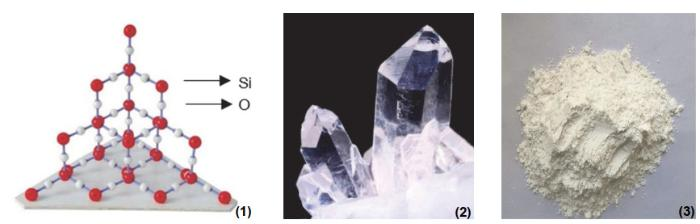
\includegraphics[width=.8\textwidth]{SiO2}\par
(1) 二氧化硅(SiO2)结构;(2) 结晶二氧化硅;(3) 无定形二氧化硅
\end{block}

\begin{block}[width=.9\textwidth]{\refname}
\printbibliography[heading=none]
\end{block}

\end{frame}
\end{document}
